\documentclass{beamer}
\usepackage{chronosys}

\usepackage{ifpdf}
\ifpdf
\usepackage{hyperref}
%\pdfadjustspacing=1
%\fi

\mode<presentation>
 {
  \usetheme{Frankfurt}
   \usecolortheme[rgb={0.36,0.54,0.66}]{structure}
   
   \definecolor{inaf}{HTML}{1D71B8}
   %\definecolor{ashgrey}{rgb}{0.7, 0.75, 0.71}
   \definecolor{autumn}{rgb}{0.7, 0.75, 0.71}
   \definecolor{autumn1}{rgb}{0.7, 0.75, 0.71}
   \definecolor{autumn2}{rgb}{0.36, 0.54, 0.66}
   
   \definecolor{blue}{HTML}{84CECC}
   \definecolor{gr}{HTML}{375D81}

\setbeamercolor{alerted text}{fg=inaf!80!yellow}
\setbeamercolor*{palette primary}{fg=inaf!60!black,bg=autumn}
\setbeamercolor*{palette secondary}{fg=white!70!black,bg=autumn2}
\setbeamercolor*{palette tertiary}{bg=white!80!black,fg=autumn2}
\setbeamercolor*{palette quaternary}{fg=white,bg=autumn2}

\setbeamercolor*{sidebar}{fg=inaf,bg=autumn}

\setbeamercolor*{palette sidebar primary}{fg=inaf!10!black}
\setbeamercolor*{palette sidebar secondary}{fg=white}
\setbeamercolor*{palette sidebar tertiary}{fg=inaf!50!black}
\setbeamercolor*{palette sidebar quaternary}{fg=yellow!10!orange}

\setbeamercolor*{titlelike}{parent=palette primary}
\setbeamercolor{frametitle}{bg=autumn1}
\setbeamercolor{frametitle right}{bg=autumn}

\setbeamercolor*{separation line}{}
\setbeamercolor*{fine separation line}{}

\mode
<all>
   
   %\usecolortheme{wolverine}
   \usecolortheme{rose}
   \usefonttheme{serif}
%   \setbeamercolor{section in toc}{fg=red}
 }

\title[Astronomia planetaria]{Astronomia planetaria:\\transiti ed esopianeti in classe}
\author[G.Filippelli]{Gianluigi Filippelli}
\date{Liceo "C. Cavalleri", Parabiago (Milano). 29/11/2017}

\usepackage[latin1]{inputenc}
\usepackage[italian]{babel}
\usepackage{times}
%
\begin{document}
%
\begin{frame}
 \titlepage
\end{frame}
%
% Inizio
%
\section{Gli inizi}
%
\begin{frame}[tolomeo]
	\frametitle{Il sistema tolemaico}
	\begin{center}
		{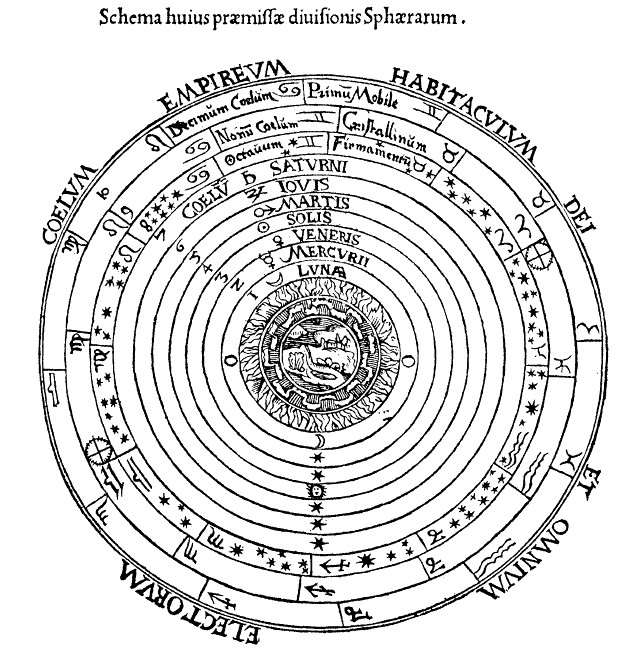
\includegraphics[width=6cm]{files/tolomeo.jpg}}
	\end{center}
\end{frame}
%
\begin{frame}[giordanobruno]
	\frametitle{Altrimondi}
	\begin{center}
		{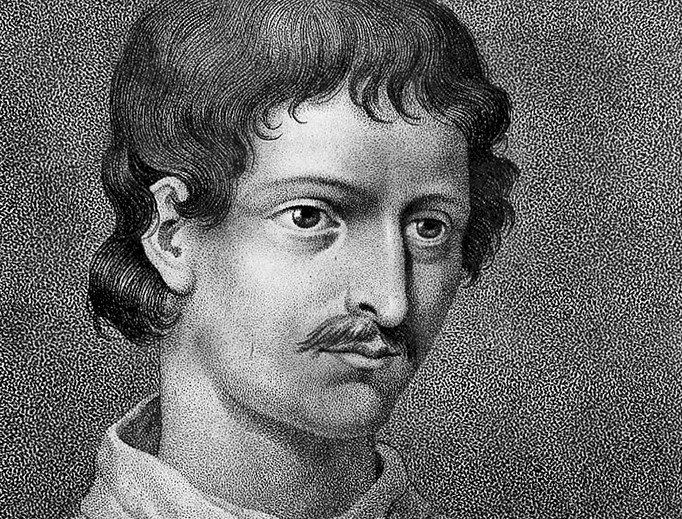
\includegraphics[width=6cm]{files/giordanobruno.jpg}}
	\end{center}
\end{frame}
%
\begin{frame}[timeline01]
	\frametitle{Una timeline: il primo presunto esopianeta}
	%---------------------timeline----------------%
	\startchronology[align=left, startyear=1915,stopyear=1935, height=0pt, startdate=false, stopdate=false, dateselevation=0pt, arrow=false, box=true]
	%
	\chronograduation[event][dateselevation=0pt]{1}
	%---------------------periods----------------%
	\chronoperiode[textstyle=\raggedleft\colorbox{inaf!50}, color=gr, startdate=false, bottomdepth=0pt, topheight=8pt, textdepth=-25pt,dateselevation=16pt, stopdate=false]{1917}{1918}{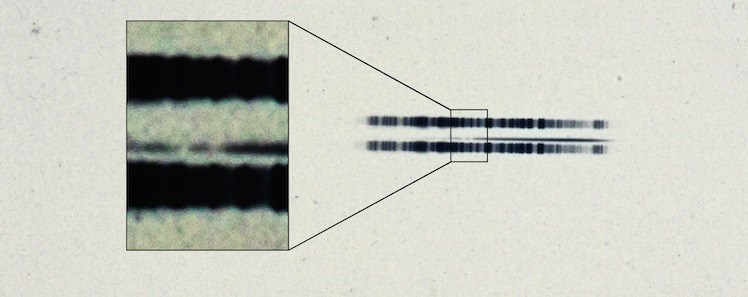
\includegraphics[width=4cm]{files/vanmaanen2.jpg}}
	%
	\stopchronology
	\begin{itemize}
		\item Spettro di van Maanen 2; nel riquadro le linee associate con gli elementi sulla superficie della stella via  \href{https://goo.gl/TMU2nG}{\textcolor{inaf}{Phil Plait}}
	\end{itemize}
\end{frame}
%
\begin{frame}[timeline03]
	\frametitle{Una timeline: le prime osservazioni}
	%---------------------timeline----------------%
	\startchronology[align=left, startyear=1980,stopyear=1996, height=0pt, startdate=false, stopdate=false, dateselevation=0pt, arrow=false, box=true]
	%
	\chronograduation[event][dateselevation=0pt]{1}
	%---------------------periods----------------%
	\chronoperiode[textstyle=\raggedleft\colorbox{inaf!50}, color=gr, startdate=false, bottomdepth=0pt, topheight=8pt, textdepth=-25pt,dateselevation=16pt, stopdate=false]{1983}{1984}{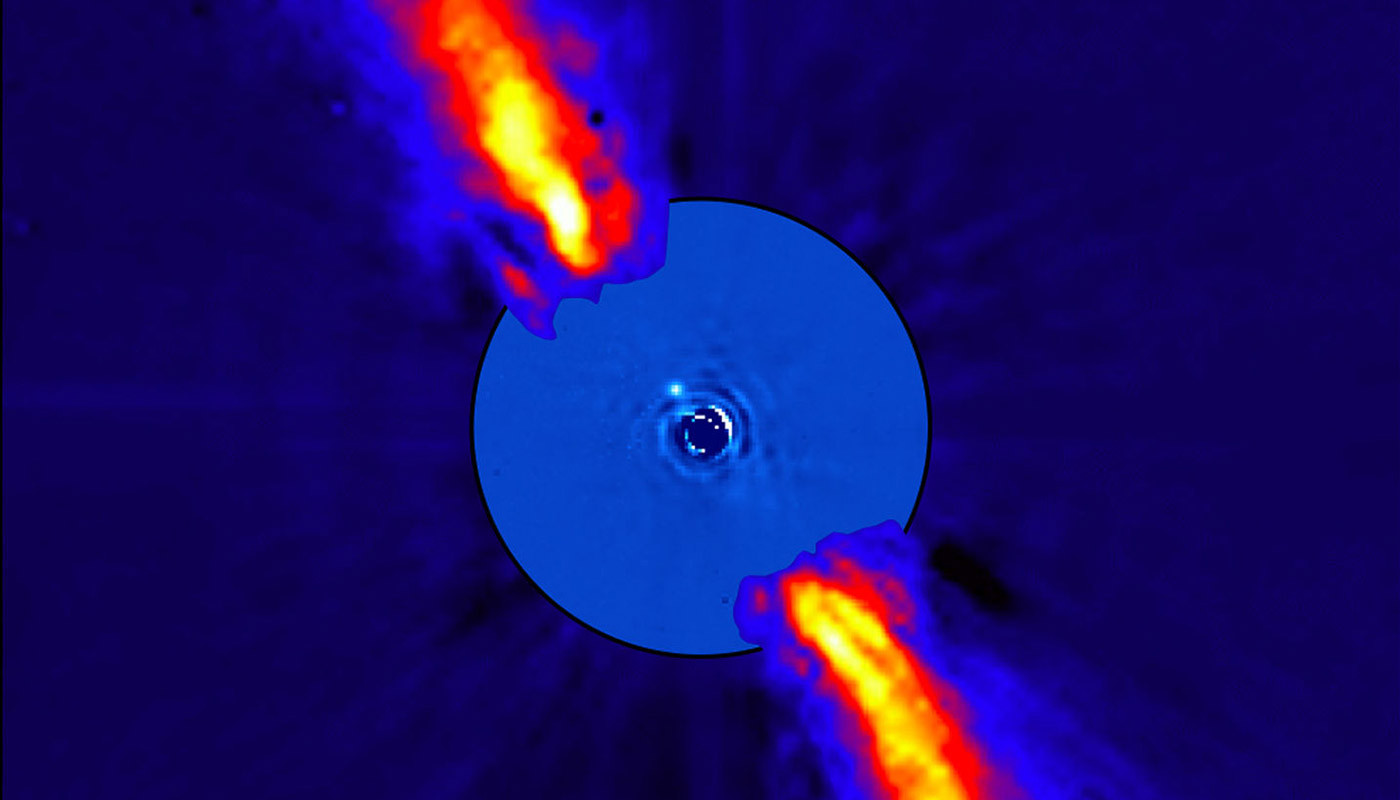
\includegraphics[width=4cm]{files/planetarydisc.jpg}}
	%
	\stopchronology
	\begin{itemize}
		\item Prima osservazione di un disco planetario
	\end{itemize}
\end{frame}
%
\begin{frame}[timeline03]
	\frametitle{Una timeline: le prime osservazioni}
	%---------------------timeline----------------%
	\startchronology[align=left, startyear=1980,stopyear=1996, height=0pt, startdate=false, stopdate=false, dateselevation=0pt, arrow=false, box=true]
	%
	\chronograduation[event][dateselevation=0pt]{1}
	%---------------------periods----------------%
	\chronoperiode[textstyle=\raggedleft\colorbox{gr!50}, color=gr, startdate=false, bottomdepth=0pt, topheight=8pt, textdepth=-25pt,dateselevation=16pt, stopdate=false]{1983}{1984}{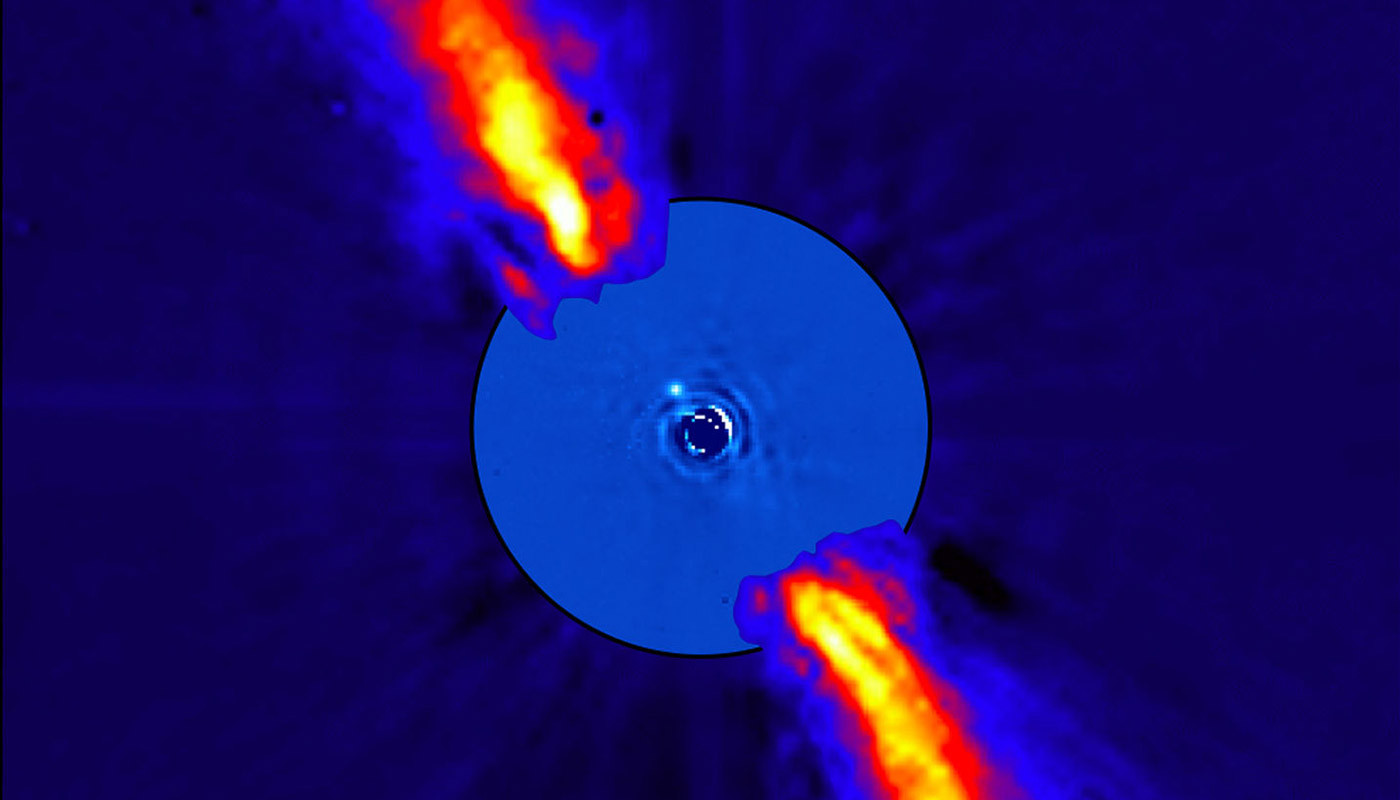
\includegraphics[width=4cm]{files/planetarydisc.jpg}}
	%
	\chronoperiode[textstyle=\raggedleft\colorbox{inaf!50}, color=gr, startdate=false, bottomdepth=0pt, topheight=8pt, textdepth=-25pt,dateselevation=16pt, stopdate=false]{1988}{1989}{Gamma Cephei Ab}
	%
	\stopchronology
	\begin{itemize}
		\item Esistenza del pianeta confermata nel 2002
	\end{itemize}
\end{frame}
%
\begin{frame}[timeline04]
	\frametitle{Una timeline: le prime osservazioni}
	%---------------------timeline----------------%
	\startchronology[align=left, startyear=1980,stopyear=1996, height=0pt, startdate=false, stopdate=false, dateselevation=0pt, arrow=false, box=true]
	%
	\chronograduation[event][dateselevation=0pt]{1}
	%---------------------periods----------------%
	\chronoperiode[textstyle=\raggedleft\colorbox{gr!50}, color=gr, startdate=false, bottomdepth=0pt, topheight=8pt, textdepth=-25pt,dateselevation=16pt, stopdate=false]{1983}{1984}{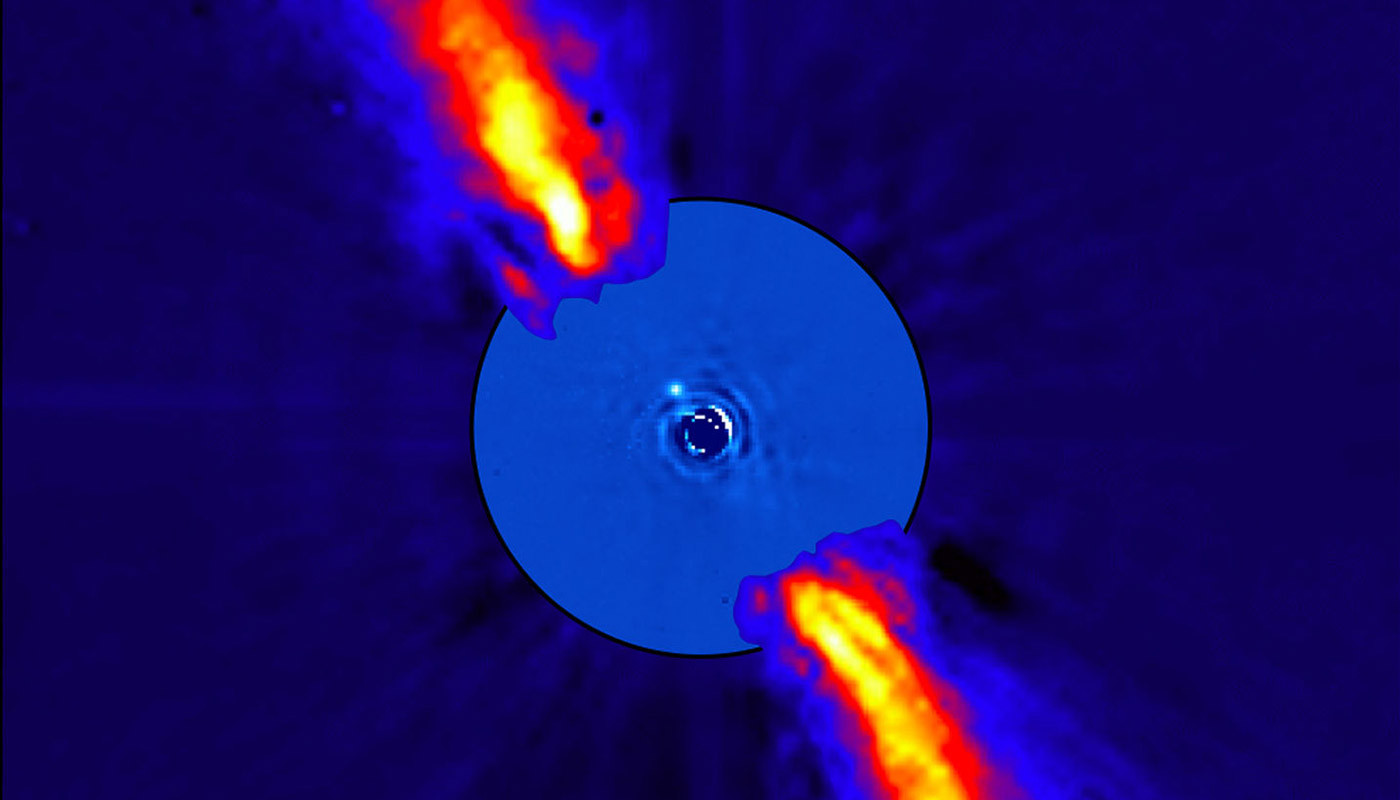
\includegraphics[width=4cm]{files/planetarydisc.jpg}}
	%
	\chronoperiode[textstyle=\raggedleft\colorbox{gr!50}, color=gr, startdate=false, bottomdepth=0pt, topheight=8pt, textdepth=-25pt,dateselevation=16pt, stopdate=false]{1988}{1989}{Gamma Cephei Ab}
	%
	\chronoperiode[textstyle=\raggedleft\colorbox{inaf!50}, color=gr, startdate=false, bottomdepth=0pt, topheight=8pt, textdepth=-25pt,dateselevation=16pt, stopdate=false]{1995}{1996}{51 Pegasi b}
	%
	\stopchronology
	\begin{itemize}
		\item Il primo esopianeta a essere confermato come tale. Orbita intorno a una stella nella sequenza principale
	\end{itemize}
\end{frame}
%
\subsection{La prima osservazione ottica}
\begin{frame}[ottica]
	\frametitle{Una timeline: la prima osservazione ottica}
	%---------------------timeline----------------%
	\startchronology[align=left, startyear=2000,stopyear=2017, height=0pt, startdate=false, stopdate=false, dateselevation=0pt, arrow=false, box=true]
	%
	\chronograduation[event][dateselevation=0pt]{1}
	%---------------------periods----------------%
	\chronoperiode[textstyle=\raggedleft\colorbox{inaf!50}, color=gr, startdate=false, bottomdepth=0pt, topheight=8pt, textdepth=-25pt,dateselevation=16pt, stopdate=false]{2004}{2005}{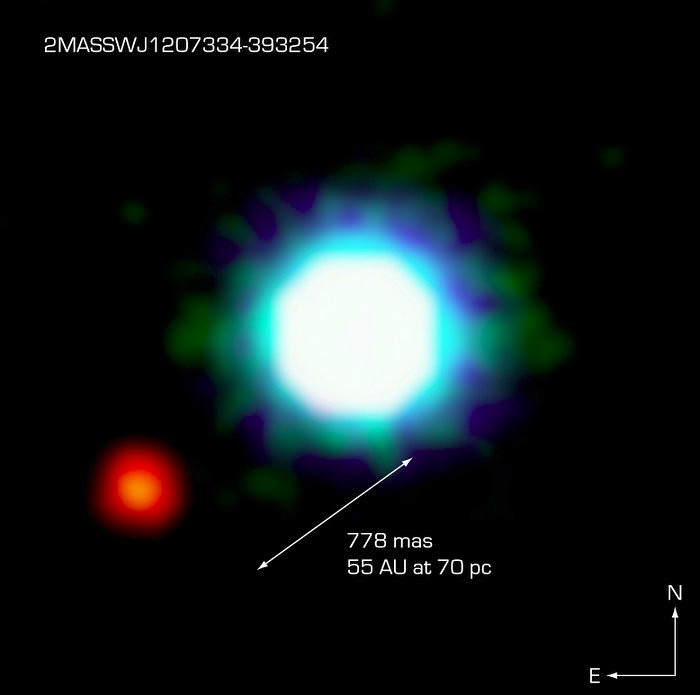
\includegraphics[width=4cm]{files/exoplanet_vlt.jpg}}
	%
	\stopchronology
	\begin{itemize}
		\item La prima osservazione di un esopianeta \href{https://www.eso.org/public/news/eso0428/}{\textcolor{inaf}{fatta dal VLT}} via \href{http://www.syfy.com/syfywire/first-exoplanet-image-confirmed}{\textcolor{inaf}{Phil Plait}}
	\end{itemize}
\end{frame}
%
% Velocit� radiale
%
\section{Metodi di rilevazione}
\subsection{Oscillazione Doppler}
\begin{frame}[doppler01]
	\frametitle{Velocit� radiale o oscillazione Doppler}
	\scriptsize
	\onslide<1->
	\begin{block}{Ipotesi}
		La velocit� radiale di una stella � influenzata dalla presenza di un pianeta in orbita intorno alla stessa.
	\end{block}
	\onslide<2->
	\begin{block}{Cosa osservare}
		La velocit� radiale proveniente dalla stella sar� tendente al blu quando il pianeta sulla sua orbita si muove verso la Terra, sar� tendente al rosso quando il pianeta si allontana.
	\end{block}
\end{frame}
%
\begin{frame}[doppler02]
	\frametitle{Velocit� radiale o oscillazione Doppler}
	\scriptsize
	\onslide<1->
	\begin{block}{Vantaggi}
		Efficace per rilevare pianeti massicci.
	\end{block}
	\onslide<2->
	\begin{block}{Difficolt�}
		Difficolt� nel determinare l'esatta orbita di un pianeta e quindi il periodo di rotazione orbitale e l'eccentricit�.
	\end{block}
\end{frame}
%
\subsection{Transito}
\begin{frame}[transito01]
	\frametitle{Metodo del transito: un'infografica}
	\begin{center}
		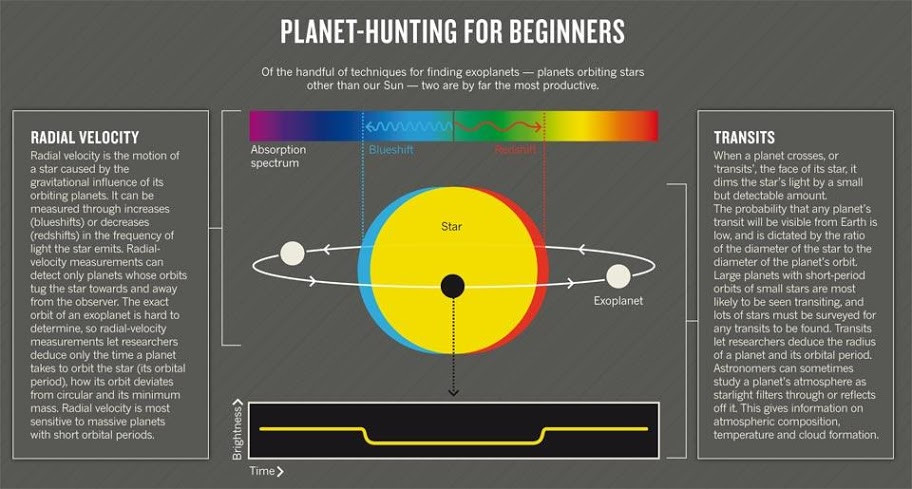
\includegraphics[width=8cm]{files/transitbeginners.jpg}
	\end{center}
\end{frame}
%
\begin{frame}[transito02]
	\frametitle{Metodo del transito}
	\begin{block}{Cosa osservare}
		Si studia l'intensit� della luce emessa dalla stella (la luminosit�): quando la luce diminuisce, questo vuol dire che davanti alla stella sta passando un oggetto.
	\end{block}
	\begin{block}{Vantaggi}
		Si possono determinare: il raggio dell'oggetto e il suo periodo orbitale. Inoltre � anche possibile studiarne l'atmosfera, la sua composizione, la temperatura e l'eventuale presenza e formazione di nuvole.
	\end{block}
\end{frame}
%
\subsection{Missione Kepler}
\begin{frame}[kepler01]
	\frametitle{Kepler: l'esposione degli esopianeti}
	\begin{center}
		{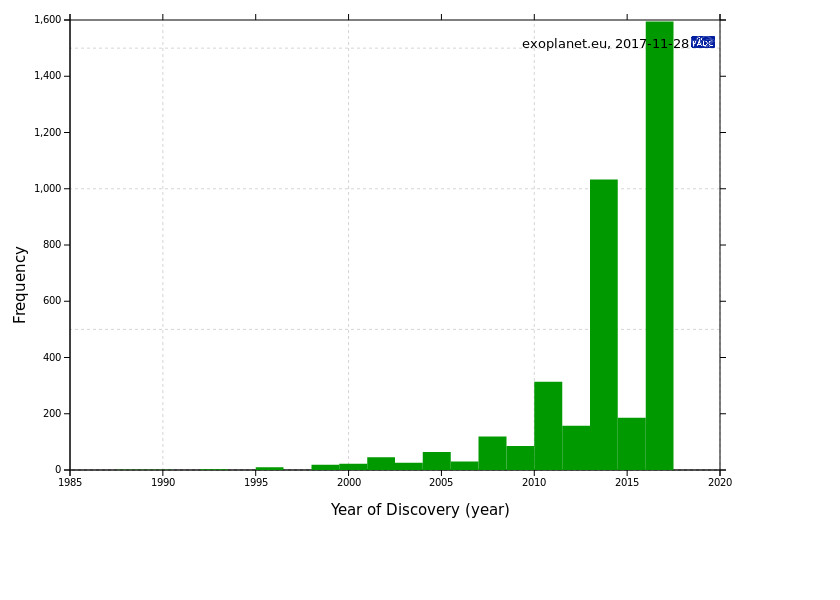
\includegraphics[width=8cm]{files/exoplanets.jpg}}
	\end{center}
\end{frame}
%
\begin{frame}[exoplanets]
	\frametitle{Kepler: grafici dai dati reali}
	\begin{center}
		{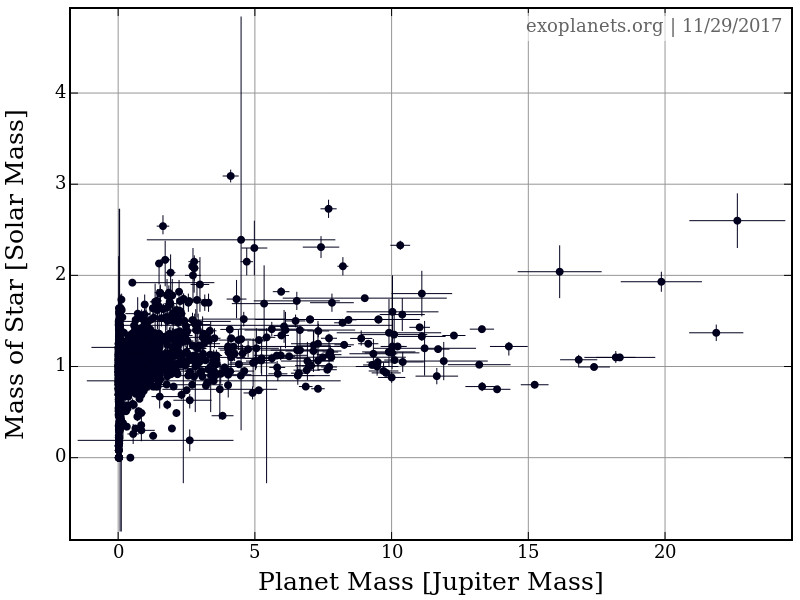
\includegraphics[width=8cm]{files/planets_vs_stars.jpg}}
	\end{center}
\end{frame}
%
\section{La velocit� radiale in classe}
\begin{frame}[velocita]
	\frametitle{Un po' di trigonometria}
	\begin{block}{Eccentricit�}
		\[r' = a \frac{1-e^2}{1+e \cos \left ( 2\pi \frac{t}{p}\right )}\]
		$a$ semi asse maggiore, $e$ eccentricit�, $r'$ raggio orbitale del pianeta, $p$ periodo orbitale
	\end{block}
	LoPresto, M., McKay, R. (2005). An introductory physics exercise using real extrasolar planet data \emph{Physics Education}, 40 (1), 46-50 DOI: \href{http://dx.doi.org/10.1088/0031-9120/40/1/003}{\textcolor{inaf}{10.1088/0031-9120/40/1/003}} (\href{http://www.df.uba.ar/users/sgil/physics_paper_doc/papers_phys/extra_planetary.pdf}{\textcolor{inaf}{pdf}})
\end{frame}
%
\section{Il transito in classe}
\begin{frame}[kepler02]
	\frametitle{Kepler: utilizzare i dati}
	\begin{block}{Studio diretto dei dati astronomici}
		Pubblici e liberamente consultabili (generalmente dopo 6 mesi), alcuni anche in formati semplici da leggere anche con gli usuali \emph{editor} di testo. Ci� permette di confrontarsi con dati reali e alla loro elaborazione statistica.
	\end{block}
\end{frame}
%
\begin{frame}[kepler03]
	\frametitle{Kepler: un po' di matematica}
	\begin{block}{Il raggio del pianeta}
		La profondit� del transito
		\[\Delta F = \frac{B_{\text{max}} - B_{\text{min}}}{B_{\text{max}}}\]
		� direttamente proporzionale a
		\[\left(\frac{R_p}{R_s}\right)^2\]
		dove $B_{\text{max}}$, $B_{\text{min}}$ sono rispettivamente le intensit� luminose prima/dopo e durante il transito; $R_s$, $R_p$ rispettivamente i raggi della stella e del pianeta
	\end{block}
\end{frame}
%
\begin{frame}[kepler04]
	\frametitle{Kepler: un po' di matematica}
	\begin{block}{Le dimensioni dell'orbita}
		La durata del transito
		\[\tau = \frac{RP}{\pi a}\]
		� legata al raggio della stella $R$, al periodo orbitale $P$, al raggio medio dell'orbita $a$.\\
		L'equazione precedente, data $v_c$ la velocit� circolare del pianeta, � ricavata dal confronto tra
		\[P = \frac{2 \pi a}{v_c}\]
		\[\tau = \frac{2R}{v_c}\]
	\end{block}
\end{frame}
%
\begin{frame}[kepler05]
	\frametitle{Kepler: un po' di matematica}
	\begin{block}{La massa della stella}
		\[P = \frac{2 \pi}{\sqrt{G M_s}} a^{\frac{3}{2}}\]
		con $P$ periodo orbitale, $M_s$ massa della stella, $a$ raggio medio dell'orbita
	\end{block}
\end{frame}
%
\begin{frame}[kepler]
	\frametitle{Kepler: simulare il transito in laboratorio}
	\begin{center}
		{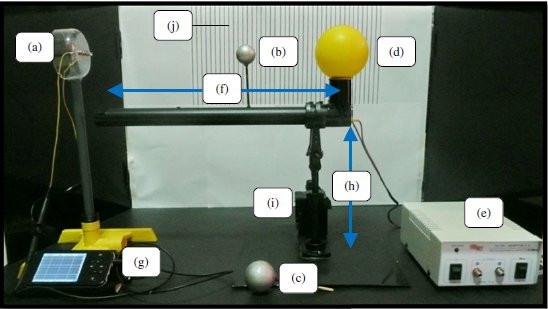
\includegraphics[width=6cm]{files/setup.jpg}}
	\end{center}
\end{frame}
%
\section{Bibliografia}
%
\begin{frame}[bibliografia]
	\frametitle{Bibliografia}
	\begin{itemize}
		\item \href{https://exoplanets.nasa.gov/alien-worlds/historic-timeline/}{\textcolor{inaf}{Timeline della NASA sulla ricerca degli esopianeti}}
		\item \href{http://exoplanet.eu/diagrams/?t=h}{\textcolor{inaf}{Grafici con i dati di Kepler}}
		\item \href{http://exoplanets.org/}{Exoplanet Orbit Database}
		\item Edu INAF: \href{http://edu.inaf.it/index.php/attivita_didattica/una-simulazione-della-missione-kepler/}{\textcolor{inaf}{Una simulazione della missione Kepler}}
		\begin{itemize}
			\item \href{http://dropseaofulaula.blogspot.it/2012/03/simulare-il-transito-di-pianeti.html}{\textcolor{inaf}{Simulare il transito di pianeti extrasolari}}
			\item Choopan, W., Ketpichainarong, W., Laosinchai, P., Panijpan, B. (2011). A demonstration setup to simulate detection of planets outside the solar system \emph{Physics Education}, 46 (5), 554-558 DOI: \href{http://dx.doi.org/10.1088/0031-9120/46/5/007}{\textcolor{inaf}{10.1088/0031-9120/46/5/007}}
			\item George, S. (2011). Extrasolar planets in the classroom Physics Education, 46 (4), 403-406 DOI: \href{http://dx.doi.org/10.1088/0031-9120/46/4/004}{\textcolor{inaf}{10.1088/0031-9120/46/4/004}} (\href{https://arxiv.org/abs/1103.5690}{\textcolor{inaf}{arXiv}})
		\end{itemize}
	\end{itemize}
\end{frame}
\end{document}
